%=================================================================
% MTI manuscript — SHORTENED VERSION (target 15-16 pages).
%
% Differences from main.tex, all requested by the supervisor:
%   * abstract under 250 words and much lighter on results
%   * contribution 4 (real-time / detection-bound) replaced by the JAAD
%     cross-dataset validation; latency survives as a supporting result
%   * new Section 4 "Experimental Settings" (hardware, software, all model
%     settings), with the hyperparameter table moved into it
%   * figure captions cut to two or three lines
%   * Discussion has no subsections
% main.tex is unchanged. Compile: tectonic main_short.tex
%=================================================================
\documentclass[mti,article,submit,moreauthors]{Definitions/mdpi}

% MDPI internal commands - do not modify
\firstpage{1}
\makeatletter
\setcounter{page}{\@firstpage}
\makeatother
\pubvolume{1}
\issuenum{1}
\articlenumber{0}
\pubyear{2026}
\copyrightyear{2026}
\datereceived{ }
\dateaccepted{ }
\datepublished{ }
\externalbibliography{yes}

% Float placement. LaTeX's defaults reserve so much of a page for text that a
% page carrying two large floats is left half empty; with 6 figures and 5 tables
% that cost several pages of white space. These are the standard relaxations and
% they change only where floats sit, never the content.
\renewcommand{\topfraction}{0.92}
\renewcommand{\bottomfraction}{0.85}
\renewcommand{\textfraction}{0.06}
\renewcommand{\floatpagefraction}{0.80}
\setcounter{topnumber}{3}
\setcounter{bottomnumber}{2}
\setcounter{totalnumber}{4}

%=================================================================
% Full title
\Title{Two Streams, Four Architectures: A Leakage-Free, Statistically Rigorous Benchmark for Pedestrian Crossing-Intention Prediction on PIE}

% Authors (PLACEHOLDER — to be completed by the authors)
\newcommand{\orcidauthorA}{0000-0000-0000-000X}
\Author{Firstname Lastname $^{1,}$*\orcidA{} and Firstname Lastname $^{1}$}

\AuthorNames{Firstname Lastname and Firstname Lastname}

% Affiliations (PLACEHOLDER)
\address{%
$^{1}$ \quad Affiliation; department, university, city, country; e-mail@e-mail.com}

\corres{Correspondence: e-mail@e-mail.com}

% Abstract (no blank lines) — 199 words
\abstract{Anticipating whether a pedestrian is about to cross is central to the safety of advanced driver-assistance and automated-driving systems, and the Pedestrian Intention Estimation (PIE) dataset has become the standard benchmark for the task. We show that the windowing protocol in common use on PIE frequently admits the crossing event into the observation window, so that for much of the positive class the benchmark measures detection rather than prediction. Auditing the protocol against PIE's own per-frame annotations quantifies the problem, and we therefore re-extract observation windows anchored at PIE's crossing-point event with a strictly pre-onset horizon, obtaining a protocol with no verified leakage and, as a side effect, several times the data. On that protocol we evaluate a deliberately parsimonious model consuming only a pedestrian bounding box and the ego-vehicle's speed, subjecting it to bootstrap and pedestrian-cluster confidence intervals, leave-one-set-out cross-validation, multi-seed ablations, a documented hyperparameter search, and a detector-in-the-loop test. We then train four temporal architectures through one identical engine with matched search budgets, separating the contribution of the input representation from that of the encoder, and replicate both the audit and the architecture comparison on a second dataset. The results identify which of the two design choices actually carries this~task.}

% Keywords
\keyword{pedestrian crossing intention; intention prediction; PIE dataset; JAAD dataset; temporal leakage; BiLSTM; Transformer; ego-vehicle speed; ADAS; cross-dataset validation}

\begin{document}

%=================================================================
\section{Introduction}

The World Health Organization estimates 1.19 million road traffic deaths in 2021 and reports that road traffic injury remains the leading cause of death for people aged 5--29 years~\citep{who2023roadsafety}. Pedestrians carry a share of that burden out of proportion to the protection afforded them, accounting for 23\% of road traffic fatalities globally, second only to occupants of four-wheeled vehicles (Figure~\ref{fig:stats}a). In the United States, 7,314 pedestrians were killed in 2023, roughly 49\% above the 4,910 recorded in 2014, and the pedestrian share of all traffic fatalities climbed from 15\% to 18\% over that decade (Figure~\ref{fig:stats}b)~\citep{nhtsa2025pedestrians}. Vehicles have become markedly safer for the people travelling inside them without becoming correspondingly safer for those in front of them.

How this risk distributes matters as much as its size. In 2023, 84\% of United States pedestrian fatalities occurred in urban areas, 74\% away from intersections, and 77\% in the dark~\citep{nhtsa2025pedestrians}: the typical fatal encounter is not a signalled crosswalk at midday but an unsignalled crossing in city traffic and poor light. Advanced driver-assistance systems (ADAS) must therefore anticipate a crossing \emph{before} it begins, since braking distance at urban speeds consumes most of the interval between recognition and impact.

\begin{figure}[htbp]
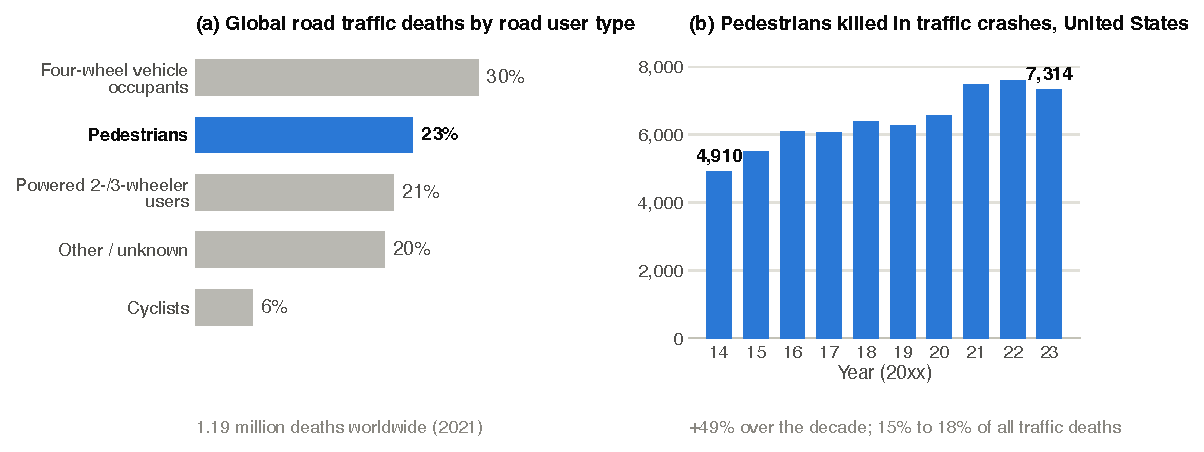
\includegraphics[width=\textwidth]{figures/fig1_pedestrian_statistics.pdf}
\caption{Pedestrians carry a disproportionate and growing share of road traffic casualties. (\textbf{a}) Global road traffic deaths by road user type, 2021~\citep{who2023roadsafety}. (\textbf{b}) Pedestrians killed in the United States, 2014--2023~\citep{nhtsa2025pedestrians}.\label{fig:stats}}
\end{figure}

This is the task of pedestrian crossing-intention prediction: from a short observation of a pedestrian and of the ego-vehicle, estimate the probability that the pedestrian is about to cross~\citep{rasouli2019pie,kotseruba2021benchmark}. It is not trajectory forecasting, which extrapolates motion that has already begun; an intention model must commit to a binary, safety-critical decision while the pedestrian is still on the kerb, under substantial class imbalance. The Pedestrian Intention Estimation (PIE) dataset~\citep{rasouli2019pie} pairs on-board video with per-frame bounding boxes, per-pedestrian crossing labels, and synchronized on-board-diagnostics (OBD) ego-vehicle speed, and most subsequent models are compared on its fixed split by recording set.

Despite the maturity of this benchmark, three methodological weaknesses recur. First, \textbf{temporal leakage is rarely checked}. Many PIE protocols anchor the observation window at the last annotated frame minus a fixed time-to-event offset, with no guarantee that the window ends before the pedestrian begins to cross; when it overlaps frames in which the pedestrian is already crossing, the task quietly collapses from predicting an intention to detecting an event in progress. The dataset authors' own benchmark notes a related misalignment between how intention and action samples are anchored~\citep{rasouli2024diving}, but a direct, quantified audit is, to our knowledge, absent. Second, \textbf{recent models are heavy}: three to seven input streams require pose estimators, optical-flow networks, segmentation, or depth models at inference time, which raises cost and is awkward on embedded automotive hardware~\citep{azarmi2025pipnet,xie2025gtranspdm}. Third, \textbf{evaluation is often thin}, resting on single splits, single-seed ablations reported as conclusions, point estimates without intervals, ground-truth boxes substituted for a real detector, and unjustified hyperparameters~\citep{rasouli2024diving,azarmi2024featureimportance}.

We do not claim that minimal-modality prediction is itself new; Section~\ref{sec:relatedwork} reviews the prior work establishing it. What has been missing is a demonstration that it survives a leakage-free protocol and full statistical scrutiny, together with an explanation of \emph{why} so few inputs suffice.

Our contributions are:
\begin{itemize}
\item A quantified \textbf{temporal-leakage audit} of the common PIE protocol and a \textbf{leakage-free re-extraction} anchored at PIE's own crossing point, verified at 0\% window leakage (Sections~\ref{sec:leakage} and~\ref{sec:leakage-results}).
\item A \textbf{rigorous re-evaluation} of a parsimonious two-stream (bounding box + ego-speed) model: bootstrap and pedestrian-cluster intervals, leave-one-set-out cross-validation, multi-seed ablations, a documented hyperparameter search, and a detector-in-the-loop test (Section~\ref{sec:results}).
\item A \textbf{four-family architecture study}. A bidirectional LSTM, a searched Transformer, a GRU, and an un-gated vanilla RNN, trained under one identical engine with matched search budgets, prove statistically indistinguishable on the primary metric, so \textbf{the input signal, not the architecture or its gating, decides} (Section~\ref{sec:architecture}).
\item A \textbf{cross-dataset replication on JAAD} showing that the leakage is not PIE-specific and that, with leakage removed and no ego-speed channel, all four families fall to chance, corroborating the input-signal claim and bounding its scope (Section~\ref{sec:jaad}).
\end{itemize}

Throughout we adopt the metric hierarchy \textbf{F1 $\rightarrow$ accuracy $\rightarrow$ AUC}: F1 is the imbalance-appropriate operating-point metric we report first, accuracy second, and ROC/PR-AUC as threshold-free corroboration.

%=================================================================
\section{Related Work}
\label{sec:relatedwork}

\subsection{Datasets, Benchmarks, and Models}

Research on crossing prediction has been shaped by a small set of datasets recorded from a moving vehicle. JAAD introduced short clips annotated with pedestrian actions around the moment of crossing~\citep{rasouli2017jaad}, and PIE extended this to roughly six hours of continuous urban driving with bounding-box tracks, behavioural tags, and synchronized OBD signals~\citep{rasouli2019pie}. The benchmark of~\citet{kotseruba2021benchmark} fixed how observation windows, horizons, and partitions are defined on both and released the PCPA reference model. Even so, results do not transfer cleanly: predictors trained on one dataset lose substantial accuracy on another, pointing to dataset-specific bias rather than a solved task~\citep{gesnouin2022assessing}. Two surveys map the area in more detail~\citep{sharma2022survey,rasouli2024diving}.

Early predictors borrowed sequence models from trajectory forecasting, where the LSTM~\citep{hochreiter1997lstm} and its bidirectional form~\citep{schuster1997bilstm} had proved effective for pedestrian motion. The field then developed along three lines: graph-based models representing pedestrian, scene, and relations as nodes and edges, from Pedestrian Graph+~\citep{cadena2022pedgraph} to models that treat a group of pedestrians jointly~\citep{zou2025group}; attention- and transformer-based models that augmented or replaced recurrence, including CAPformer~\citep{lorenzo2021capformer}, IntFormer~\citep{lorenzo2021intformer}, PIT~\citep{zhou2023pit}, PedFormer~\citep{rasouli2023pedformer}, and GTransPDM~\citep{xie2025gtranspdm}; and progressive modality fusion, from PCPA's visual, motion, and ego cues~\citep{kotseruba2021benchmark} to PIP-Net's seven concurrent streams including depth and optical flow~\citep{azarmi2025pipnet}. Recent work adds uncertainty-aware and diffusion formulations~\citep{chen2024pedcmt,liu2025occlusion}, contextual feature fusion~\citep{azarmi2023local}, neuro-symbolic reasoning for explainability~\citep{melocastillo2025neurosymbolic}, and multi-context or sequential-plus-visual transformers~\citep{li2025mft,landry2025trajfusionnet,liang2024tcl}. Sensing beyond the on-board camera has also been tried, including infrastructure-side prediction at intersections~\citep{abdelrahman2025vrucipi}.

\subsection{Minimal-Modality Prediction and the Perception Front End}

The prevailing trend adds modalities to chase accuracy, but a counter-current asks whether they earn their cost. The transformer backbone behind most recent models is expensive to run~\citep{vaswani2017attention}, and a crossing predictor must fit inside a tight frame budget on embedded hardware; lighter recurrent units such as the GRU~\citep{cho2014gru} were partly motivated by that pressure. Several works establish that a minimal input is surprisingly strong. \citet{achaji2022attention} report 91\% accuracy and 0.83 F1 on PIE from box geometry alone, though as Section~\ref{sec:leakage} shows those numbers were measured under the pre-leakage protocol. Closest to our design, PedCMT predicts crossing from \emph{only} the bounding box and ego-vehicle speed within a cross-modal transformer, on a par with models using more inputs~\citep{chen2024pedcmt}, and the pose-free ablation of GTransPDM reaches comparable accuracy from the same two streams~\citep{xie2025gtranspdm}. We take minimal inputs as an established design choice and ask how far two cheap streams go once the evaluation is made leakage-free and statistically strict, and \emph{why} they suffice.

Most studies evaluate on ground-truth boxes, which skips the perception stage any deployed system must include. In practice a predictor receives boxes from a single-stage detector of the YOLO family~\citep{jocher2025yolo} and identities from a tracking-by-detection method such as ByteTrack~\citep{zhang2022bytetrack}. We pair the two to measure how a real front end affects prediction (Section~\ref{sec:detector}).

\subsection{Pedestrian--Vehicle Interaction and Remaining Gaps}

Crossing is an interaction, not a solitary act. A substantial body of work studies how automated vehicles signal intent through external human--machine interfaces and how those signals change crossing decisions~\citep{alhawiti2024ehmi,rezwana2024interactions}. That literature concerns \emph{explicit} communication from vehicle to pedestrian; our result points the other way and complements it. The ego-vehicle's speed profile carries much of the predictive signal, which makes the vehicle's own motion an \emph{implicit} channel a model can read, while also cautioning that a model leaning on ego-speed partly reads the driver's anticipation rather than the pedestrian alone.

A fourth gap joins the three set out in the Introduction: the modalities that matter are seldom isolated. A context-aware feature-importance analysis finds that bounding box and ego-speed dominate, and cautions that reliance on ego-speed can induce a driver-side bias in yielding scenarios~\citep{azarmi2024featureimportance}. Together these four gaps organize the rest of the paper.

%=================================================================
\section{Materials and Methods}
\label{sec:methods}

\subsection{Overview}

The study has a deliberately narrow design. One dataset, one windowing protocol, one input representation, and one training engine are held fixed; only the factors under test vary, namely the window anchoring rule, the presence of the ego-speed stream, the temporal encoder, the observation length, and the prediction horizon. Everything outside the dashed block of Figure~\ref{fig:system}a is frozen, which is what allows a difference between two rows of a results table to be attributed to a single design choice.

\begin{figure}[htbp]
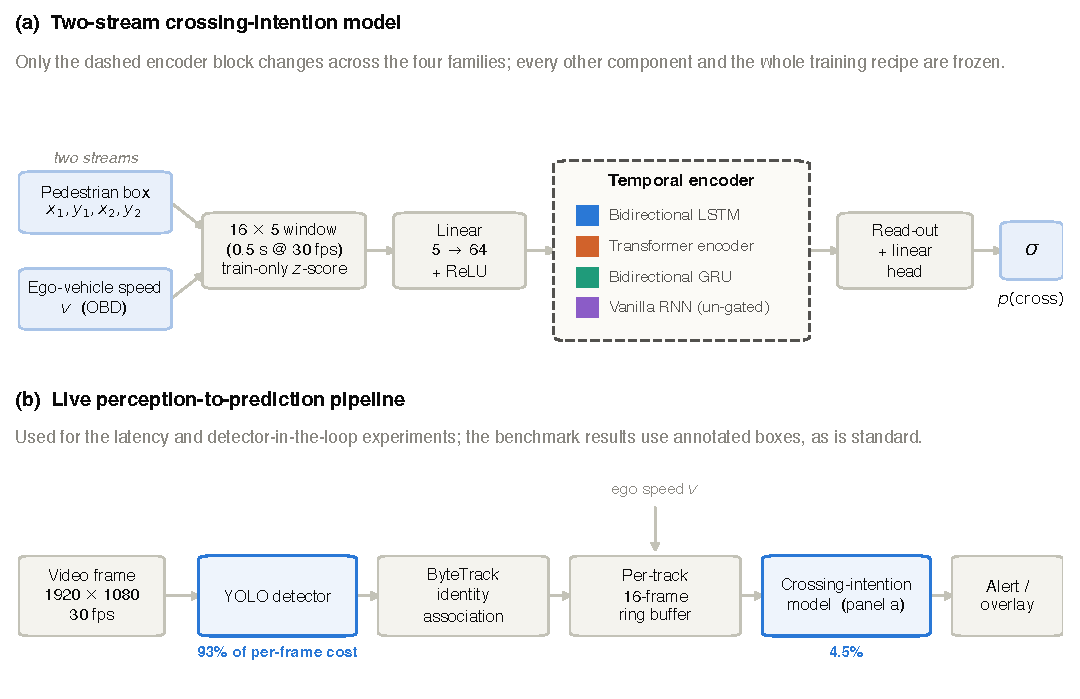
\includegraphics[width=\textwidth]{figures/fig2_system.pdf}
\caption{The model and the pipeline it runs inside. (\textbf{a}) The two-stream crossing-intention model; only the dashed encoder block changes across the four families. (\textbf{b}) The live perception-to-prediction pipeline, annotated with each stage's measured share of per-frame cost.\label{fig:system}}
\end{figure}

\subsection{The PIE Dataset and Splits}
\label{sec:dataset}

PIE~\citep{rasouli2019pie} comprises roughly six hours of on-board video (1920$\times$1080 at 30\,fps) recorded in Toronto traffic across six recording sets. Each annotated pedestrian carries a per-frame bounding-box track, a per-frame \texttt{cross} state, a binary crossing label and, critically for this work, a \texttt{crossing\_point} event frame marking when the crossing begins. Ego-vehicle speed is recorded synchronously from the OBD port, giving a second modality available at inference time without additional perception. We use the standard benchmark split by recording set (train set01/02/04, validate set05/06, test set03), which prevents identity- and scene-level leakage because a pedestrian, a video, and a stretch of road each belong to exactly one split, and which is the partition used by the reference benchmark~\citep{kotseruba2021benchmark} and by our baselines.

\subsection{Temporal Leakage and the Leakage-Free Protocol}
\label{sec:leakage}

The prevailing extraction procedure places each observation window at the last annotated frame of a pedestrian's track, minus a fixed time-to-event (TTE) offset. The difficulty is that the end of an annotated track has no defined relationship to the moment the pedestrian steps into the road: a track may continue for many seconds after the crossing begins, in which case a window offset backwards from its end still lands well inside the crossing (Figure~\ref{fig:protocol}a), and the task silently changes from predicting an intention to recognizing an event in progress. PIE's per-frame \texttt{cross} attribute lets this be measured directly; we re-parsed the annotation XML to recover that state and used it as ground truth for the audit in Section~\ref{sec:leakage-results}.

The fix follows from the diagnosis: measure backwards from the event rather than from the end of a track. For each pedestrian we take the contiguous track segment containing \texttt{crossing\_point}, truncate it at that frame inclusive, and slide 16-frame windows across the remaining history at 50\% overlap, keeping only those whose last observed frame falls a TTE of $[30, 60]$ frames (1--2\,s) \emph{before} the crossing point (Figure~\ref{fig:protocol}b). Non-crossing pedestrians contribute windows from their full track under the same length and stride, and pedestrians whose usable track is shorter than the window plus the minimum look-ahead (107 of 1,374, or 7.8\%) are excluded.

Two properties make this leakage-free by construction rather than by inspection: \texttt{crossing\_point} coincides with the first frame labelled \texttt{cross}~=~\emph{crossing} for 516 of 519 crossing pedestrians (99.4\%) and never precedes it, and requiring 30 frames of look-ahead puts the last observed frame at least a full second before that marker. Table~\ref{tab:dataset} summarizes what changes; the leakage-free protocol also yields 3.5 times the data, because it slides windows across pre-crossing history rather than taking one per track.

\begin{table}[htbp]
\caption{Track-end versus crossing-point anchoring on PIE. Re-anchoring removes all window leakage and grows the sample 3.5-fold. Window counts are total (train/validation/test); the class weight is the training loss's positive-class weight, the training split's negative-to-positive ratio.\label{tab:dataset}}
\begin{tabularx}{\textwidth}{lCCCC}
\toprule
\textbf{Protocol} & \textbf{Windows} & \textbf{Positive Rate} & \textbf{Window Leakage} & \textbf{Class Weight}\\
\midrule
Track-end anchor & 1389 \newline (616/186/587) & 41.0\% & 387/570 (67.9\%) & 1.44\\
\textbf{Crossing-point} & 4906 \newline (2178/634/2094) & 33.6\% & \textbf{0/4906 (0.0\%)} & 1.682\\
\bottomrule
\end{tabularx}
\end{table}

\begin{figure}[htbp]
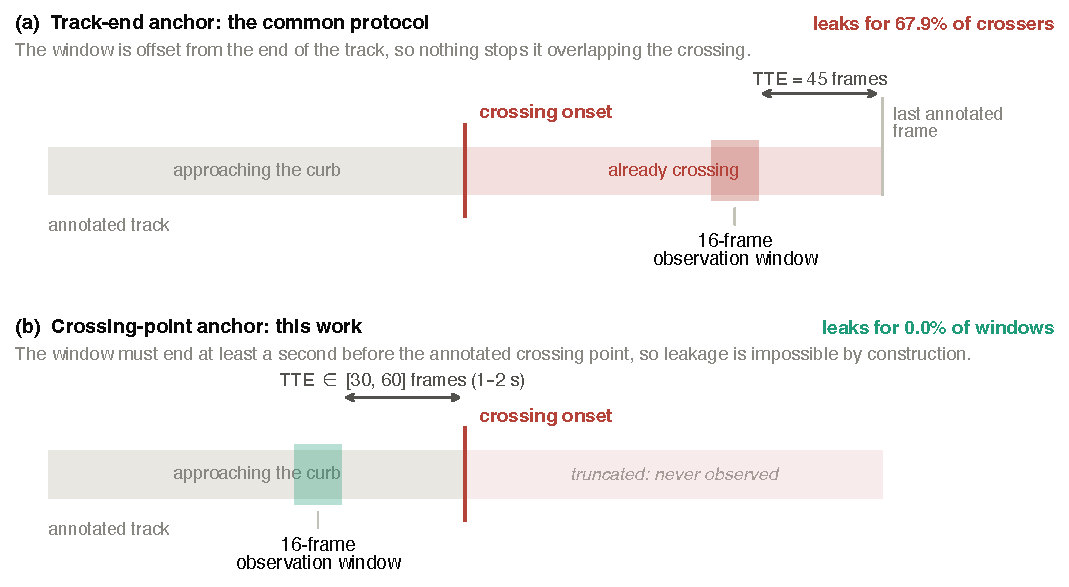
\includegraphics[width=\textwidth]{figures/fig3_protocol.pdf}
\caption{Where the observation window lands under each anchoring rule. (\textbf{a}) A track-end anchor places no constraint on the onset, so the window may overlap the crossing. (\textbf{b}) Anchoring at \texttt{crossing\_point} with a 30--60 frame look-ahead makes leakage impossible.\label{fig:protocol}}
\end{figure}

\subsection{Features and Preprocessing}
\label{sec:features}

Every model receives the same input: a 16-frame window (0.5\,s at 30\,fps) of a five-dimensional vector $[x_1, y_1, x_2, y_2, v]$, where $(x_1, y_1, x_2, y_2)$ are the pedestrian's bounding-box corners and $v$ is the ego-vehicle speed. Box coordinates are kept in raw PIE pixel units on the 1920$\times$1080 image plane and deliberately \emph{not} normalized by image size, so the network sees absolute geometry. Each feature is standardized by its own $z$-score with $\mu$ and $\sigma$ computed on the training split alone, since computing them over the whole dataset would leak distributional information about the evaluation sets. The ablation of Section~\ref{sec:ego-ablation} drops $v$ and is otherwise identical. Unless stated otherwise the decision threshold is 0.5 on the sigmoid output, which makes our numbers directly comparable with the baselines in Table~\ref{tab:baselines}.

\subsection{Model Architectures}
\label{sec:architectures}

All four families share one minimal wrapper: a linear projection of the five input features to 64 dimensions with a ReLU nonlinearity, a temporal encoder, a read-out of the final or pooled time step, and a linear head producing a single logit. Only the encoder differs, and every network is trained from scratch.

The \textbf{BiLSTM} is a two-layer bidirectional long short-term memory network~\citep{hochreiter1997lstm} with last-step read-out, and is the reference and headline system. The \textbf{Transformer} is a small pre-layer-norm encoder~\citep{vaswani2017attention} whose width, depth, head count, pooling, and positional encoding were searched. The \textbf{GRU} is the BiLSTM with its cell replaced by a gated recurrent unit~\citep{cho2014gru} and nothing else changed, isolating \emph{which} gated cell is used; the \textbf{vanilla RNN} is the BiLSTM with gating removed entirely, a bidirectional tanh (Elman) network~\citep{elman1990rnn}, isolating \emph{gating itself}. The three recurrent families therefore form a ladder: if recurrent machinery is what makes this task work, performance should fall at each rung. Two further BiLSTM variants serve as ablations, a bounding-box-only model dropping the ego-speed stream and a model with additive temporal attention over the recurrent states~\citep{bahdanau2015attention}.

\subsection{Metric Hierarchy, Evaluation, and Statistical Procedure}
\label{sec:metrics}

We report F1 first, accuracy second, and ROC-AUC and PR-AUC as threshold-free corroboration. The ordering suits an imbalanced, safety-critical binary decision: a deployed system must commit to a threshold, so a metric summarizing performance at an operating point is more informative than one averaging over all of them, and with roughly one window in three positive, accuracy alone rewards a model leaning toward the majority class. AUC still checks whether an F1 result is an artifact of threshold placement. Making F1 primary has three consequences, applied symmetrically to all four families: $\tau$ is tuned on validation data only, each configuration is re-selected by validation F1, and checkpoints are taken at best validation F1. Models selected under the older AUC-first rule are labelled as such.

Point estimates are per-seed means over five seeds, and every claim of a difference is backed by an interval from a 10,000-resample bootstrap on the 2,094 test windows. Windows from the same pedestrian are not independent, since they overlap in time and share an identity, a scene, and a behaviour, so a bootstrap that resamples windows understates uncertainty; we therefore also report a \emph{pedestrian-cluster} bootstrap that resamples the 541 test pedestrians as whole units and treat that stricter interval as the primary evidence. Comparisons between models are \emph{paired} bootstraps on identical resamples, which removes the shared difficulty of the test set from the contrast. Generalization beyond the fixed split is assessed by leave-one-set-out (LOSO) cross-validation across all six recording sets. A five-seed probability ensemble, where reported, is labelled as such.

\subsection{Live Perception-to-Prediction Pipeline}
\label{sec:pipeline}

For the deployment analysis we built the pipeline of Figure~\ref{fig:system}b. Pedestrians are detected with a YOLO-family single-stage detector~\citep{jocher2025yolo}, associated across frames by ByteTrack~\citep{zhang2022bytetrack}, and buffered per track into the same 16-frame window of $[x_1, y_1, x_2, y_2, v]$ the offline models consume, with $v$ read from the vehicle rather than from vision. It supplies the latency measurement (Section~\ref{sec:loso}), the detector-in-the-loop experiment (Section~\ref{sec:detector}), and the qualitative examples (Section~\ref{sec:qualitative}); the benchmark results use annotated boxes, as every comparable study does.

%=================================================================
\section{Experimental Settings}
\label{sec:settings}

\subsection{Computing Environment}

Model training under the clean protocol, all statistical analysis, the recurrent-family hyperparameter searches, and every timing measurement were carried out locally on an Apple M4 system-on-chip (10 CPU cores, 16\,GB unified memory) running macOS~26.5. The larger Transformer search and the observation-length sweeps ran on a Kaggle cloud instance with an NVIDIA Tesla T4 GPU (16\,GB). Every configuration appearing in a results table was retrained locally through the same engine, so no reported number depends on which machine produced it, and inference parity was verified at approximately $10^{-6}$ absolute difference in output probability.

The software stack was Python 3.13.5 with PyTorch 2.12.0~\citep{paszke2019pytorch}, NumPy 2.4.6, SciPy 1.17.1, and scikit-learn 1.9.0 for metrics and statistical tests. The perception front end used Ultralytics 8.4.68 with a YOLO26-M detector and the bundled ByteTrack implementation.

One reproducibility caveat is worth recording. Training \texttt{nn.LSTM} on Apple's Metal Performance Shaders backend proved dependent on process history, so the same configuration and seed can produce different results depending on what ran earlier in the same process. Recurrent runs that must reproduce exactly were therefore executed on CPU, where training is bit-reproducible; Transformer training did not show this behaviour.

\subsection{Training Configuration}

Every family is trained through a single model-agnostic engine, so the recipe cannot drift between architectures. The loss is binary cross-entropy with a positive-class weight of 1.682, the training split's negative-to-positive ratio, applied only in the training gradient. Optimization uses Adam~\citep{kingma2015adam} with weight decay $10^{-5}$ (decoupled in the Transformer recipe-search stage), batch size 32, at most 100 epochs, early stopping with patience 15, and a plateau schedule that halves the learning rate after five epochs without validation improvement. Every configuration is trained with five seeds (42, 0, 1, 2, 3). The test set is evaluated exactly once per model, on the checkpoint selected by validation performance, by a single designated script that is the only code path with test access.

\subsection{Hyperparameter Search and Selected Settings}

Hyperparameters are searched rather than asserted, and the search is reported whether or not it changed anything. The BiLSTM received a 36-configuration grid, fixed a priori, over learning rate $\{10^{-3}, 5{\cdot}10^{-4}, 10^{-4}\}$, dropout $\{0.2, 0.3, 0.5\}$, hidden size $\{64, 128, 256\}$, and depth $\{1, 2\}$, the 54 nominal cells collapsing to 36 because inter-layer dropout is inert at a single layer. Selection ran in three stages: all 36 at seed 42 ranked by validation performance, then the top five plus the baseline across five seeds, then the winner and baseline trained with five seeds and the test set touched once. The GRU and the vanilla RNN each received the \emph{identical} budget. The Transformer, having more architectural freedom, received a 78-configuration staged search over width $\{(64,128), (128,256), (128,512)\}$, depth $\{2, 4\}$, pooling $\{\text{cls}, \text{mean}, \text{last}\}$, and positional encoding $\{\text{learned}, \text{sinusoidal}\}$, followed by a recipe stage over learning rate, schedule, dropout, and weight decay. No stage evaluated the test set. This symmetry matters more than the searches individually, since a comparison in which one family is tuned and another is not measures tuning effort rather than architecture. Table~\ref{tab:hparams} lists the selected settings.

\begin{table}[htbp]
\caption{Selected settings per headline model; everything not listed is identical across families (Section~\ref{sec:settings}). ``Width'' is the recurrent hidden size, read-out being twice this, or the Transformer's model and feed-forward dimensions; $\tau$ is tuned on validation only.\label{tab:hparams}}
\begin{tabularx}{\textwidth}{Llccccc}
\toprule
\textbf{Model} & \textbf{Cell} & \textbf{Width} & \textbf{Layers} & \textbf{Drop.} & \textbf{LR} & \textbf{$\tau$}\\
\midrule
BiLSTM (baseline) & LSTM & 128 & 2 & 0.3 & $10^{-3}$ & 0.50\\
BiLSTM-F1 & LSTM & 256 & 2 & 0.3 & $10^{-3}$ & 0.52\\
Transformer (searched) & attention (4 heads) & 128/512 & 4 & 0.1 & $10^{-3}$ & 0.50\\
Transformer-F1 & attention (4 heads) & 128/512 & 4 & 0.1 & $10^{-3}$ & 0.65\\
GRU-F1 & GRU & 256 & 2 & 0.3 & $5{\cdot}10^{-4}$ & 0.53\\
Vanilla RNN-F1 & Elman (tanh) & 256 & 2 & 0.2 & $10^{-4}$ & 0.53\\
\bottomrule
\end{tabularx}
\end{table}

%=================================================================
\section{Results}
\label{sec:results}

\subsection{The Temporal-Leakage Audit}
\label{sec:leakage-results}

Auditing the track-end protocol against the recovered per-frame \texttt{cross} state gives the paper's first finding. Of 570 crossing pedestrians, 387 (67.9\%) have at least one frame inside the observation window in which they are already crossing and 369 (64.7\%) are crossing in \emph{all sixteen}; only 183 (32.1\%) have a clean window (Figure~\ref{fig:leakage}a). The median gap between the end of the window and the crossing onset is $+182$ frames, six seconds \emph{into} the crossing. For roughly two-thirds of the positive class, what is reported as prediction is the detection of an event already under way.

A static shortcut accompanies the leakage. The single bounding box at the last observed frame separates the classes on its own, with no temporal information at all: rank-biserial correlations of $+0.65$ for box area, $+0.63$ for height, and $+0.49$ for the bottom edge (Figure~\ref{fig:leakage}b), as expected of pedestrians already in the road and therefore nearer the camera. Models trained on this protocol converged by epoch~3. The identical audit on the crossing-point protocol finds 0 of 4,906 windows leaking and every static effect below 0.3 (area 0.25, height 0.21, bottom edge 0.09), so whatever signal remains must live in temporal dynamics.

\begin{figure}[htbp]
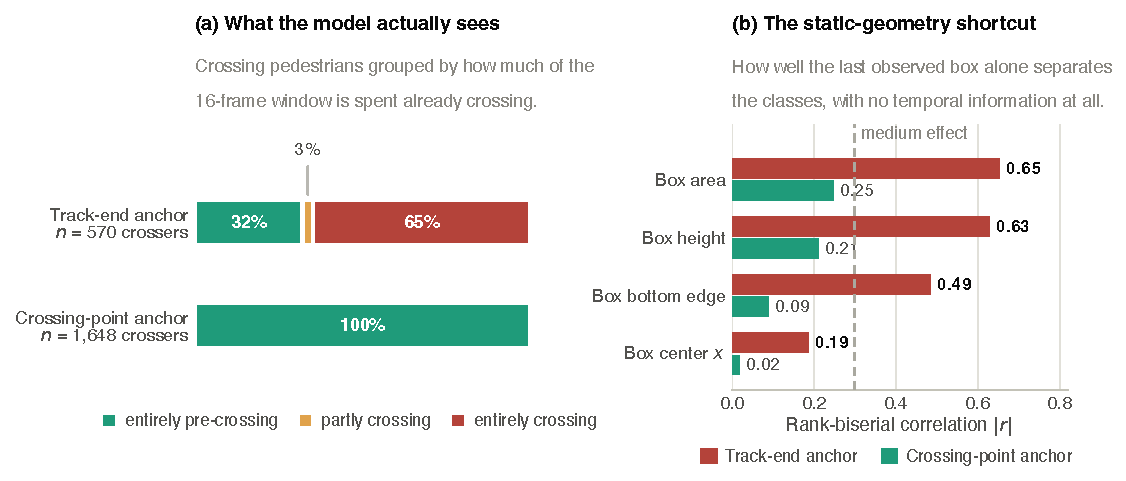
\includegraphics[width=\textwidth]{figures/fig4_leakage.pdf}
\caption{The temporal-leakage audit, from PIE's own per-frame \texttt{cross} annotations. (\textbf{a}) Crossers grouped by how much of the window is already spent crossing. (\textbf{b}) How well the last observed box alone separates the classes.\label{fig:leakage}}
\end{figure}

\subsection{Main Result}
\label{sec:main-result}

On the leakage-free protocol the two-stream BiLSTM reaches test F1 0.844, accuracy 0.897, and ROC-AUC 0.940 under F1-first optimization (Table~\ref{tab:families}), with PR-AUC 0.876 and a 95\% bootstrap AUC interval of $[0.92, 0.95]$ at the window level and $[0.92, 0.96]$ over pedestrian clusters.

Removing the leakage barely moved this model's AUC, from 0.931 on the leaky protocol to 0.932~$\pm$~0.011 over five seeds, while moving convergence from epoch~3 to a believable epoch~17; the correction is methodological rather than a deflation of the score. Nor is the new protocol simply an easier one: per-pedestrian AUC (0.914) matches per-window AUC (0.913), so the result is not an artifact of correlated windows, and the short tracks admitted by the 50\% overlap are \emph{harder} than the rest (AUC 0.863 for tracks of 46--75 frames against 0.919 for longer ones).

\subsection{Does the Architecture Matter?}
\label{sec:architecture}

Table~\ref{tab:families} reports all four families trained under the identical engine, and Figure~\ref{fig:forest} gives the paired contrasts with pedestrian-cluster intervals.

On ROC-AUC the searched Transformer is genuinely the best model in the table (0.950), and a paired bootstrap on identical test windows confirms it beats the BiLSTM ($\Delta$AUC $= +0.0135$, 95\% CI $[+0.0097, +0.0174]$). That win belongs to the search rather than to attention: the same architecture trained with the BiLSTM's own un-searched recipe merely ties it ($\Delta$AUC $= +0.0005$, interval spanning zero).

On the primary metric, however, \textbf{the four families are statistically indistinguishable}. Every cross-family $\Delta$F1 interval spans zero (Figure~\ref{fig:forest}a): GRU against BiLSTM ($+0.0071$), vanilla RNN against BiLSTM ($+0.0033$), Transformer against BiLSTM ($+0.0008$), and each remaining pair likewise. Removing the LSTM's gating entirely costs nothing over a 0.5\,s window; the un-gated network even ties the searched Transformer on AUC ($\Delta$AUC $-0.0013$, interval spanning zero) while being the smallest and fastest family in the study.

These ties are not a test without power: the same procedure detects differences where they exist, each F1-optimized model beating its own family's AUC-selected baseline by an interval clearing zero (Figure~\ref{fig:forest}a, lower group), and several AUC contrasts separating cleanly (Figure~\ref{fig:forest}b).

\begin{table}[htbp]
\caption{All four architecture families on the leakage-free PIE test set (set03; 2,094 windows, 32.5\% positive). Values are per-seed means over five seeds; ($\star$) marks each family's headline model. All models use two input streams except where noted.\label{tab:families}}
\begin{tabularx}{\textwidth}{lLcccc}
\toprule
\textbf{Family} & \textbf{Model} & \textbf{Params} & \textbf{F1} & \textbf{Acc} & \textbf{AUC}\\
\midrule
BiLSTM & BiLSTM (baseline, AUC-selected) & 594{,}561 & 0.828 & 0.883 & 0.932\\
BiLSTM & BiLSTM, bounding-box only (4-D) & 594{,}497 & 0.551 & 0.744 & 0.753\\
BiLSTM & BiLSTM + temporal attention & 611{,}265 & 0.821 & 0.879 & 0.925\\
BiLSTM & BiLSTM-F1 ($\star$) & 2{,}237{,}313 & \textbf{0.844} & 0.897 & 0.940\\
Transformer & Transformer, un-searched & 268{,}417 & 0.821 & 0.878 & 0.942\\
Transformer & Transformer, searched ($\star$) & 794{,}241 & 0.845 & 0.894 & \textbf{0.950}\\
Transformer & Transformer-F1 & 794{,}241 & 0.847 & 0.896 & 0.947\\
GRU & GRU-F1 ($\star$) & 1{,}678{,}209 & 0.849 & 0.901 & 0.941\\
RNN & Vanilla RNN-F1 ($\star$) & 560{,}001 & \textbf{0.852} & 0.902 & 0.948\\
\bottomrule
\end{tabularx}
\end{table}

\begin{figure}[htbp]
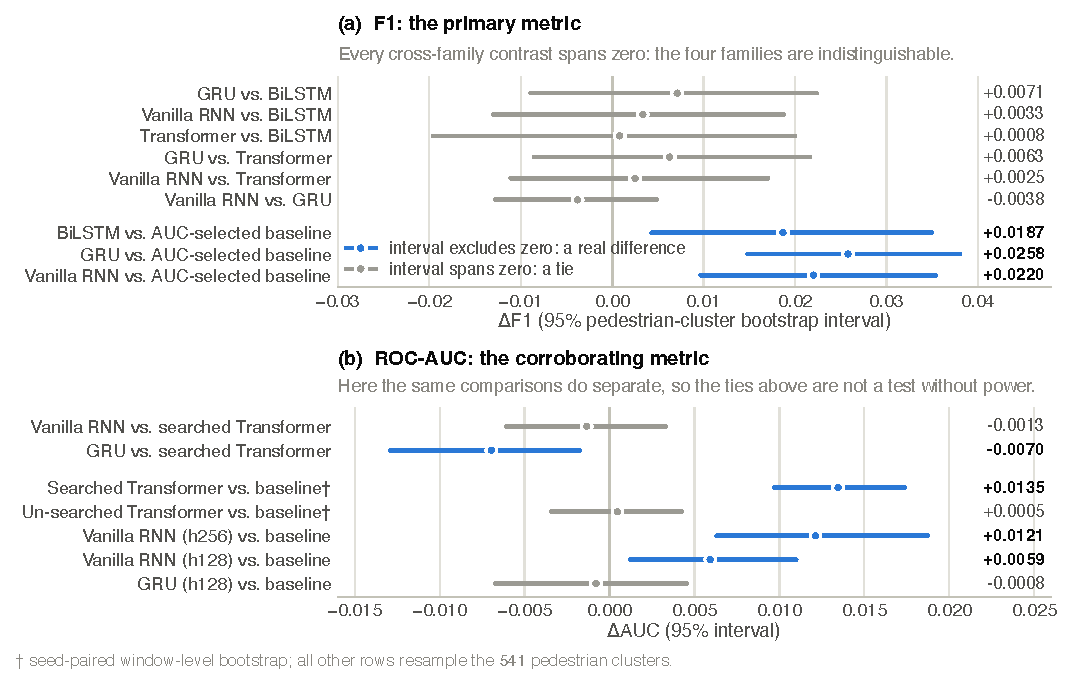
\includegraphics[width=\textwidth]{figures/fig6_forest_compact.pdf}
\caption{Paired contrasts on identical test windows, with 95\% pedestrian-cluster bootstrap intervals. (\textbf{a}) On F1 every cross-family contrast spans zero; the lower group shows the same test detecting a real effect. (\textbf{b}) On ROC-AUC the models do separate.\label{fig:forest}}
\end{figure}

\subsection{Comparison with Published Baselines}
\label{sec:baselines}

Table~\ref{tab:baselines} places our models beside published PIE results on the standard protocol, with a column counting input streams. On F1 the two-stream models reach 0.844--0.852, ahead of most multimodal baselines and within about 0.02 of the ceiling set by PedFormer (0.87), using two inputs instead of three to seven; on AUC they lead the table at 0.94--0.95; on accuracy they sit mid-band, 0.90 against PedFormer's 0.93. PIP-Net~\citep{azarmi2025pipnet} and~\citet{liu2025occlusion} are discussed but not tabulated, the first using a custom split and the second an occlusion-specific, roughly one-frame-ahead protocol.

\begin{table}[htbp]
\caption{Crossing-prediction performance on PIE under the standard protocol (train set01/02/04, validate set05/06, test set03). Baseline figures are as reported by the cited sources. Our rows are per-seed means over five seeds at threshold 0.5.\label{tab:baselines}}
\begin{tabularx}{\textwidth}{lcccL}
\toprule
\textbf{Method} & \textbf{Acc} & \textbf{AUC} & \textbf{F1} & \textbf{Modalities (Streams)}\\
\midrule
PCPA~\citep{kotseruba2021benchmark} & 0.87 & 0.86 & 0.77 & box + pose + context + speed (4)\\
Pedestrian Graph+~\citep{cadena2022pedgraph} & 0.89 & 0.90 & 0.81 & pose graph + ego (2--3)\\
IntFormer~\citep{lorenzo2021intformer} & 0.89 & 0.92 & 0.81 & multimodal\\
PIT~\citep{zhou2023pit} & 0.91 & 0.92 & 0.82 & multimodal\\
BiPed~\citep{rasouli2023pedformer} & 0.91 & 0.90 & 0.85 & multimodal\\
PedFormer~\citep{rasouli2023pedformer} & \textbf{0.93} & 0.90 & \textbf{0.87} & multimodal (multitask)\\
GTransPDM~\citep{xie2025gtranspdm} & 0.90 & 0.87 & 0.82 & box + pose + ego (3)\\
GTransPDM without pose~\citep{xie2025gtranspdm} & 0.92 & 0.90 & 0.86 & box + ego (2)\\
PedCMT~\citep{chen2024pedcmt} & 0.92 & --- & --- & box + ego-speed (2)\\
MFT~\citep{li2025mft} & 0.90 & 0.94 & 0.83 & 4 context streams\\
\midrule
BiLSTM-F1 (ours) & 0.897 & 0.940 & 0.844 & \textbf{box + ego-speed (2)}\\
Transformer-F1 (ours) & 0.896 & 0.947 & 0.847 & \textbf{box + ego-speed (2)}\\
GRU-F1 (ours) & 0.901 & 0.941 & 0.849 & \textbf{box + ego-speed (2)}\\
Vanilla RNN-F1 (ours) & 0.902 & \textbf{0.948} & \textbf{0.852} & \textbf{box + ego-speed (2)}\\
\bottomrule
\end{tabularx}
\end{table}

\subsection{Which Input Carries the Signal?}
\label{sec:ego-ablation}

Dropping the ego-speed stream from an otherwise identical BiLSTM collapses it: AUC falls from 0.932 to 0.753, F1 from 0.828 to 0.551, and accuracy from 0.883 to 0.744. A loss of 0.18 AUC from removing one of two inputs identifies ego-vehicle speed as the dominant predictor, consistent with the independent feature-importance analysis of~\citet{azarmi2024featureimportance}; adding temporal attention to the same model, by contrast, changes nothing (AUC 0.925 against 0.932). The collapse is also the other half of the leakage story, since once the static-geometry shortcut is removed a model given only bounding boxes has very little left to work with.

\subsection{Prediction Horizon and Observation Length}
\label{sec:horizon}

How far ahead the model must predict matters; how long it gets to observe does not. AUC declines monotonically as the horizon lengthens, from 0.961 at 1.0\,s to 0.946 at 1.5\,s and 0.919 at 2.0\,s, with every pairwise paired $t$-test significant ($p \le 0.004$) and Kruskal--Wallis $p = 0.002$. Because a longer horizon needs a longer usable track and so changes which pedestrians are eligible, we repeated the comparison on a matched cohort of the same 493 test pedestrians; the decline survives unchanged (sample effect $\le 0.002$ AUC). This is what one wants from a genuine predictor, and it corrects an earlier ``insensitive to horizon'' conclusion of our own that was itself a leakage artifact.

Observation length behaves in the opposite way. Over 8, 16, and 30 frames the baseline's AUC moves only from 0.931 to 0.933 to 0.937, a spread smaller than seed noise (all pairwise $p > 0.21$), and extending the window to 32 and 64 frames makes matters slightly worse for every family. Half a second already carries the available dynamics, which justifies the 16-frame window and suits deployment, since a shorter window means a shorter wait before a newly detected pedestrian can be scored. One asymmetry is worth flagging: at 64 frames the un-gated vanilla RNN alone loses 0.050 F1 against its own 16-frame result, roughly double the decline of the gated cells. Per-seed intervals overlap, so this is directional rather than bootstrap-confirmed, but the equivalence we report is horizon-bounded.


\subsection{Cross-Set Generalization, Capacity, and Latency}
\label{sec:loso}

Rotating the held-out recording set across all six folds gives an AUC of 0.928~$\pm$~0.041 with no fold collapsing. The set03 fold, our fixed test set, scores 0.931, at the fold mean rather than above it, so the headline number does not depend on set03 being an unusually easy partition; excluding only the 47-window set05 fold, too small to interpret, the remaining five give 0.915~$\pm$~0.029.

A hidden-size sweep (64, 128, 256 units giving AUC 0.927, 0.933, 0.938) and a depth sweep (1, 2, 3 layers giving 0.930, 0.932, 0.931) show the recurrent baseline is limited by data rather than capacity: hidden size 256 is not significantly better than 128 ($p = 0.34$) despite 3.8 times the parameters. The 36-configuration grid agreed, its validation winner beating the hand-set configuration on test by only $+0.0006$ ($p = 0.91$).

Latency does not discriminate among the families. On the Apple M4 CPU at batch 1 the isolated models run in 0.316--0.721\,ms per window, between 46 and 105 times inside a 30\,fps frame budget, the un-gated vanilla RNN fastest. In the full pipeline the detector accounts for about 93\% of per-frame cost and the intention model for 4.5\%, so the frame rate is a property of the detector, not of the crossing-intention model.

\subsection{Detector-in-the-Loop Robustness}
\label{sec:detector}

Benchmark numbers on PIE are computed from annotated boxes; a deployed system receives boxes from a detector. On two test-set clips covering 98 pedestrians and 311 windows, replacing annotated boxes with detector boxes (mean IoU 0.75) moved AUC only from 0.962 to 0.953 per window and from 0.958 to 0.948 per pedestrian, with the decision flipping in 10 of 311 windows (3\%): prediction is robust to realistic box noise. The weak links lie earlier. Detector recall is 88\% of pedestrians, so roughly one in eight is never covered well enough to be scored, and identity fragmentation is worse, a pedestrian's dominant ByteTrack identity covering a mean of only 39\% of its matched frames. One caveat bounds the experiment: each detector window uses the best-IoU detection per frame matched against the annotated box, which isolates localization noise but removes the association errors just quantified, so the 0.009 AUC drop is a lower bound on end-to-end degradation rather than an estimate of it.

\subsection{Qualitative Behaviour}
\label{sec:qualitative}

Figure~\ref{fig:qualitative} shows the complete pipeline on two test-set scenes, with boxes from the detector and tracker rather than from annotations and probabilities from the five-seed BiLSTM-F1 ensemble at its validation-tuned threshold of 0.516. Panel~(a) is the leakage-free protocol made visible: the model commits to ``will cross'' at $p = 0.71$ a second and a half before this pedestrian steps off the kerb. Panel~(b) is the complementary and harder case; to any rule based on position it is the same picture, a person standing at a kerb beside a marked crosswalk, but this one does not cross and the model correctly leaves him at $p = 0.31$. What separates the panels is the motion history behind each box, not where either pedestrian stands. Both are annotated in PIE, so each verdict is checked against ground truth rather than judged by eye; the frames are illustrative rather than representative, and across the two clips the ensemble scores accuracy 0.920 and F1 0.884 over 439 windows. Video~S1 shows the pipeline running continuously over 26\,s of test video.

\begin{figure}[htbp]
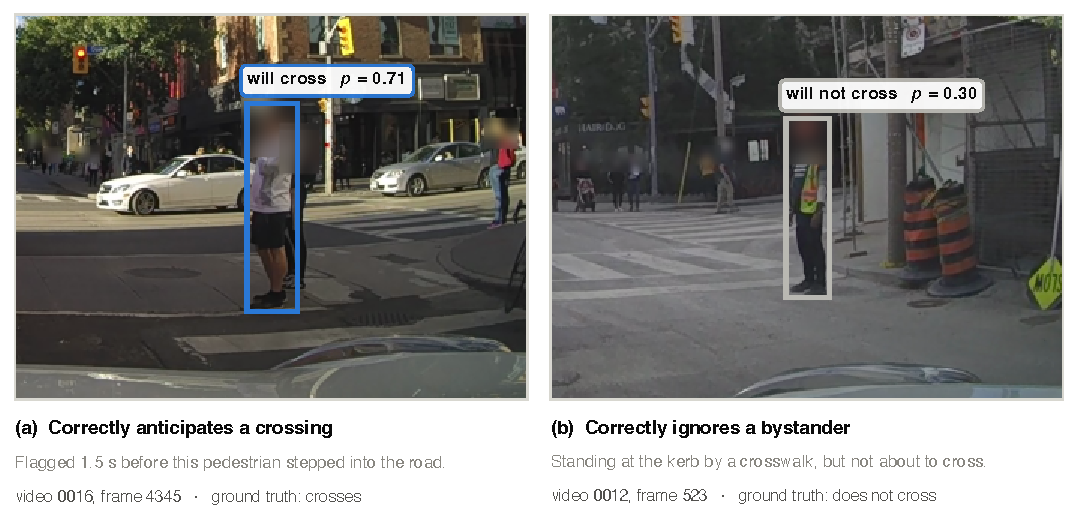
\includegraphics[width=\textwidth]{figures/fig9_qualitative.pdf}
\caption{The detection-to-prediction pipeline on two PIE test scenes, with boxes from YOLO and ByteTrack. (\textbf{a}) A pedestrian correctly flagged 1.5\,s before stepping into the road. (\textbf{b}) A worker at a kerb, correctly not flagged. Faces were blurred before publication.\label{fig:qualitative}}
\end{figure}

\subsection{Cross-Dataset Replication on JAAD}
\label{sec:jaad}

Every result above comes from one dataset, so we replicated both the audit and the architecture comparison on JAAD~\citep{rasouli2017jaad} using the same code, window, and TTE range. JAAD records no ego-vehicle speed, so a replication there tests the leakage audit and the architecture isolation but structurally cannot test the ego-speed finding, and its models run on the four-dimensional box input alone.

The leakage pathology is not PIE-specific, and on JAAD it is worse. Under a naive last-frame-minus-TTE anchor, 428 of 460 crossing pedestrians (93.0\%) have at least one already-crossing frame inside the window and 415 (90.2\%) are crossing in all sixteen, against 67.9\% and 64.7\% on PIE. The static-geometry shortcut appears at the same scale (rank-biserial $+0.48$ for box area, $+0.41$ for height, $+0.37$ for the bottom edge). Re-anchoring at the verified per-frame onset removes it completely: 0 of 972 windows leak and every static effect falls below 0.17.

The architecture comparison replicates too, but means something only once the missing modality is taken into account (Table~\ref{tab:jaad}). All four families sit at chance: test ROC-AUC ranges from 0.493 to 0.520 across families and from 0.475 to 0.558 across all twenty runs, and F1 of 0.707--0.740, though superficially healthy, is below the 0.814 a constant always-crossing prediction achieves on this 68.7\%-positive split. Without an ego-speed channel and with the static shortcut removed, none of the four learns anything from box geometry alone, and all four remain indistinguishable from one another throughout.

\begin{table}[htbp]
\caption{Cross-dataset replication on JAAD under the same leakage-free protocol, bounding-box input only (JAAD records no ego-speed). Values are means $\pm$ standard deviation over five seeds on the 399-window test split, which is 68.7\% positive. A constant always-crossing prediction would score F1 0.814 and AUC 0.500.\label{tab:jaad}}
\begin{tabularx}{\textwidth}{Llccc}
\toprule
\textbf{Family} & \textbf{Params} & \textbf{F1} & \textbf{Acc} & \textbf{AUC}\\
\midrule
BiLSTM & 594{,}497 & 0.720 $\pm$ 0.031 & 0.605 $\pm$ 0.029 & 0.510 $\pm$ 0.018\\
Transformer & 794{,}113 & 0.740 $\pm$ 0.036 & 0.619 $\pm$ 0.037 & 0.520 $\pm$ 0.020\\
GRU & 446{,}017 & 0.707 $\pm$ 0.016 & 0.584 $\pm$ 0.018 & 0.502 $\pm$ 0.020\\
Vanilla RNN & 149{,}057 & 0.729 $\pm$ 0.026 & 0.608 $\pm$ 0.028 & 0.493 $\pm$ 0.012\\
\midrule
\textit{Always-crossing baseline} & --- & \textit{0.814} & \textit{0.687} & \textit{0.500}\\
\bottomrule
\end{tabularx}
\end{table}

%=================================================================
\section{Discussion}
\label{sec:discussion}

Two cheap inputs reach F1 within about 0.02 of the multimodal ceiling and the highest AUC in the standard-protocol table, at a small fraction of the feature-extraction cost. We do not claim to be first to find this: PedCMT~\citep{chen2024pedcmt} and the pose-free ablation of GTransPDM~\citep{xie2025gtranspdm} reported comparable results from the same two streams, and~\citet{achaji2022attention} made the case from box geometry alone. What this paper adds is that the finding survives a leakage-free protocol and full statistical scrutiny, and an account of \emph{why} it holds. Removing ego-speed collapses the model, while replacing its temporal encoder with three quite different alternatives changes nothing measurable; the predictive content is therefore concentrated in the ego-speed profile and coarse box dynamics, legible within half a second, leaving no long-range structure for a heavier encoder to find. That is a claim about the task rather than about our implementation, and it explains why so many differently architected models cluster within a few points of one another. For a practitioner the implication is direct: effort spent on a pose estimator or an optical-flow network is likely better spent on the perception front end.

The architecture comparison resolves differently depending on which metric leads: on AUC a searched Transformer wins, on F1 all four families tie. Neither result is wrong, and a paper reporting only one would be telling half the story. Given the F1-first hierarchy and near-identical latency there is no performance argument for preferring a Transformer here, and several for preferring a small recurrent model. The methodological consequence is sharper: an architecture comparison reporting a single metric, from a single seed, with unequal search budgets can produce a headline in either direction. Ours could have.

That two-thirds of crossing pedestrians were observed mid-crossing under a widely used windowing rule is the most transferable finding here, and the JAAD replication strengthens it: the same convention leaks for 93.0\% of crossers on a dataset annotated by a different protocol, so the problem belongs to the convention rather than to PIE. Removing the leakage barely changed the headline AUC, which is the point rather than a reassurance, since a model scoring 0.93 by recognizing crossings in progress and one scoring 0.93 by anticipating them a second in advance are different systems that happen to share a digit. Three symptoms may help others recognize the artifact: implausibly fast convergence, epoch 3 rather than 17; static box geometry separating the classes at effect sizes above 0.6 on PIE and above 0.4 on JAAD; and insensitivity to the prediction horizon, the clearest tell, since a model that genuinely respects a horizon must find a longer one harder. The audit is cheap, needing only a per-frame event annotation both datasets already provide.

Several limitations bound these conclusions. The JAAD result is corroboration rather than confirmation: a stream worth 0.18 AUC on PIE is absent there entirely, so a dataset that cannot carry the decisive input bounds our headline claim rather than validating it, and its small clean sample makes it a weak test of any positive claim. The dominant feature is also partly a measurement of the driver, since an instrumented vehicle slows for a pedestrian the driver expects to cross; ego-speed is legitimate at inference time and available on any production vehicle, but the field has independently flagged this driver-side bias in yielding scenarios~\citep{azarmi2024featureimportance}, and a speed-perturbation study, which we have not run, is the natural next step. The equivalence is horizon-bounded, since the un-gated network begins to fall behind at a two-second window, so ``gating is unnecessary'' is a statement about half a second, not about recurrent architectures in general. The detector-in-the-loop study rests on two clips and an oracle-guided association that makes its degradation a lower bound, and seed-level statistical power is low, which is why the paired and pedestrian-cluster bootstraps carry the argument.

%=================================================================
\section{Conclusions}
\label{sec:conclusions}

We revisited pedestrian crossing-intention prediction on PIE and found that a widely used windowing protocol lets the crossing event into the observation window for 67.9\% of crossing pedestrians, turning much of the benchmark into detection rather than prediction. Re-anchoring at PIE's own crossing point removes the leakage entirely and enlarges the dataset 3.5-fold.

On that protocol a model using only a pedestrian bounding box and the ego-vehicle's speed reaches F1 0.844--0.852 and the highest AUC among published results on the standard split, with two input streams rather than the three to seven used by recent multimodal systems. Ego-speed is the dominant predictor, since removing it costs 0.18 AUC. The temporal architecture, by contrast, is close to irrelevant: a bidirectional LSTM, a searched Transformer, a GRU, and an un-gated vanilla RNN, trained under one identical engine, are statistically indistinguishable on the primary metric, and even removing gating costs nothing over a half-second window. The input signal, not the architecture, decides. No comparison rests on a point estimate; each is backed by a paired bootstrap over pedestrian clusters, with the headline model further checked by leave-one-set-out cross-validation, five-seed variance, a documented search, and a detector-in-the-loop test.

Replicating the study on JAAD shows that the leakage belongs to the windowing convention rather than to PIE, appearing there for 93.0\% of crossing pedestrians, and that without an ego-speed channel all four architectures fall to chance, as the ablation predicts. Three directions follow: cross-dataset validation of the full two-stream model, which requires a dataset carrying synchronized ego-motion; a speed-perturbation study probing how far the ego-speed result depends on the driver's anticipation; and the perception front end, since detector recall and track identity, not the intention model, would limit such a system in a vehicle.
%=================================================================
\vspace{6pt}

\supplementary{The following supporting information can be downloaded at \linksupplementary{s1}: Video S1, the detection-to-prediction pipeline running on PIE test clip video\_0012 (26\,s, annotated with per-track crossing probabilities and ego-vehicle speed).}

\authorcontributions{Conceptualization, methodology, software, validation, formal analysis, investigation, data curation, writing---original draft preparation, writing---review and editing, and visualization: [author initials]. Supervision: [supervisor initials]. All authors have read and agreed to the published version of the manuscript. (PLACEHOLDER.)}

\funding{This research received no external funding.}

\institutionalreview{Not applicable. This study used the publicly available PIE~\citep{rasouli2019pie} and JAAD~\citep{rasouli2017jaad} datasets and involved no new experiments on humans or animals. The face region of every person detected in the PIE frames reproduced in Figure~\ref{fig:qualitative} was irreversibly blurred before publication.}

\informedconsent{Not applicable.}

\dataavailability{PIE~\citep{rasouli2019pie} and JAAD~\citep{rasouli2017jaad} are publicly available. The extraction protocol, training engine, and evaluation code developed here are available from the authors on reasonable request. (PLACEHOLDER: replace with the repository URL upon release.)}

\conflictsofinterest{The authors declare no conflicts of interest.}

%=================================================================
\reftitle{References}

\bibliography{references}

\PublishersNote{}
\end{document}
